\documentclass[9pt]{llncs}
%
\usepackage{makeidx}  % allows for indexgeneration
\usepackage{graphicx}
\usepackage[T1]{fontenc} % wszyscy z pl literami
\usepackage{url}
\usepackage{multirow}
\usepackage{graphics}
\usepackage{subfigure}
\usepackage{gensymb}
\usepackage{epstopdf}
\usepackage{mathtools}
\usepackage{float}
\usepackage{sidecap}

\DeclareGraphicsExtensions{.eps}

\begin{document}
\title{Hybrid method of human limb joints positioning -- hand movement case study}
%
\author{Grzegorz Glonek \and Adam Wojciechowski}
%
\authorrunning{Grzegorz Glonek \and Adam Wojciechowski} % abbreviated author list (for running head)
%
%%%% list of authors for the TOC (use if author list has to be modified)
\tocauthor{Grzegorz Glonek, Adam Wojciechowski}
%
\institute{Institute of Computer Science\\Lodz University of Technology, Lodz, Poland,\\
	\email{grzegorz@glonek.net.pl},
	\email{adam.wojciechowski@p.lodz.pl}}

\maketitle              % typeset the title of the contribution

\begin{abstract}
	Precise and unambiguous limbs motion tracking is one of the key aspects laying behind natural human-machine communication. The paper presents a novel approach to depth sensor (Microsoft Kinect) and inertial measurement units (IMU) data fusion, providing more precise and stable hand joints tracking. The new method substitutes sensors derived joints position fusion, mainly described in literature, with sensors derived bones orientations fusion and subsequent joints positions estimation. Obtained joints positioning precision became even 25\% better than in other solutions. The paper comprises also the method evaluation results. It was verified both against professional motion tracking VICON system and Kalkbrener method \cite{Kalkbrenner2014}, the most relevant to presented solution.
\end{abstract}

\section{Introduction}
\label{sec:introduction}
Limb motion tracking, understood as an unambiguous and delay minimizing process of limb's joints 3D space position estimation, is a valid problem invaluable for current researches on Natural User Interface design. It is used nowadays in several areas such as entertainment (games and movies animations), interaction with scene objects in augmented reality systems or motor skills rehabilitation. This last area, supported by the computer system, constitutes a part of a wider subject named tele--rehabilitation.\\
For several years, the only possibility to obtain the limb joints tracking desired accuracy was to exploit professional motion capture systems i.e. VICON or Optitrack. However, since couple of years, there appear broadly available (and cheaper) devices (i.e. game controllers) that allow to track selected aspects of human motion at user's home. On the other hand, nonprofessional solutions reveal several imprecisions and constraints that might be compensated by an appropriate controllers derived data fusion.\\
In the paper two types of such devices were taken into consideration: Microsoft  Kinect 360 -- a RGB--D camera that is able to track whole human body and inertial measurement units (IMU) consisting of accelerometer and gyroscope sensors that are able to measure linear acceleration and angular speed. As the devices recording frequencies are limited (30 Hz for Kinect and 70 Hz for IMU) and the context of rehabilitation and hand gesture controlled object manipulation is considered, the hand tracking accuracy is superior to the speed of hand movement.\\
Though several authors \cite{Bo2011,Destelle2014,Murray-Smith2014} have proved that Kinect and IMU data fusion assures limbs joints positions tracking accuracy of about 2.5 -- 3 cm, presented method achieves better results --- 2 -- 2.5 cm.

\section{State of art}
Considered sensors have several measurement characteristics that should be taken into consideration during the fusion. Microsoft Kinect controller loses its tracking ability due to body parts occlusion \cite{Asteriadis2013}. Moreover, while tracking, lost joints may affect the tracking accuracy of those which are fully visible to the sensor's camera. The rotation of user body might be an example of such scenario. Basing on author's experiments, if the user rotates more than 50 degrees (angle between user and camera view directions), occluded shoulder joints (and almost half of the body) will be invisible to the device and measurements of visible parts will be unstable.\\
Another important characteristic is that joints positions measurement accuracy change with the distance between the human and the device \cite{Khoshelham2012}. Figure  \ref{fig:kinectDist} shows how estimated accuracy change with a distance. As the most important IMU flaws, the gyroscope measurement drift and the temperature related bias in accelerometer measurements may be indicated \cite{Woodman2007,Nikolic2013}. The temperature influence on bias is presented in a figure \ref{fig:imuTemp}.\\ 
The studied paper \cite{Obdrzalek2012} estimates Microsoft Kinect general posture estimation variability in range 5 -- 10 cm. Moreover, the author pointed out that the length of tracked bones vary between measurement frames in range 2 -- 5 cm.\\

\begin{figure}[H]
	%\centering   
	%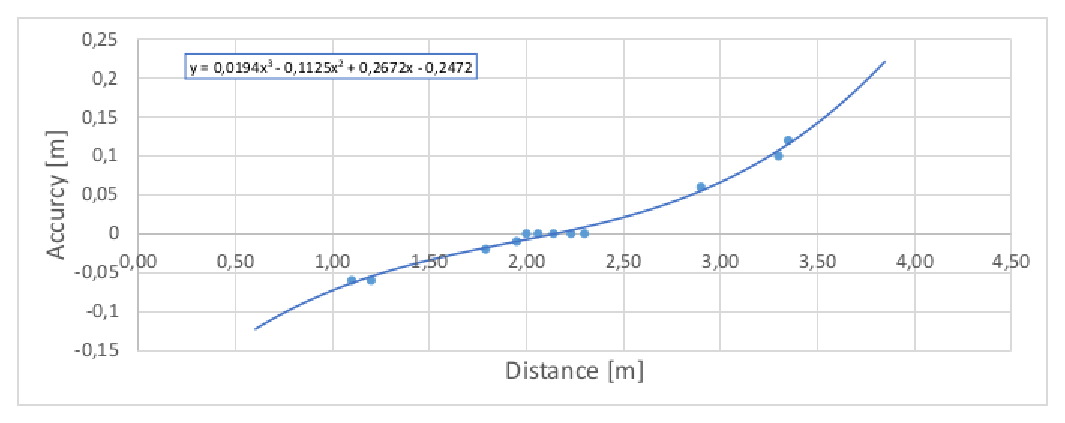
\includegraphics[width=0.45\textwidth]{Fig01.eps}
	\vspace{2.5cm}
	\caption{Position measurement accuracy in Z-axis to distance from the Kinect}
	\label{fig:kinectDist}
\end{figure}

\begin{figure}[H]
	%\centering 
	%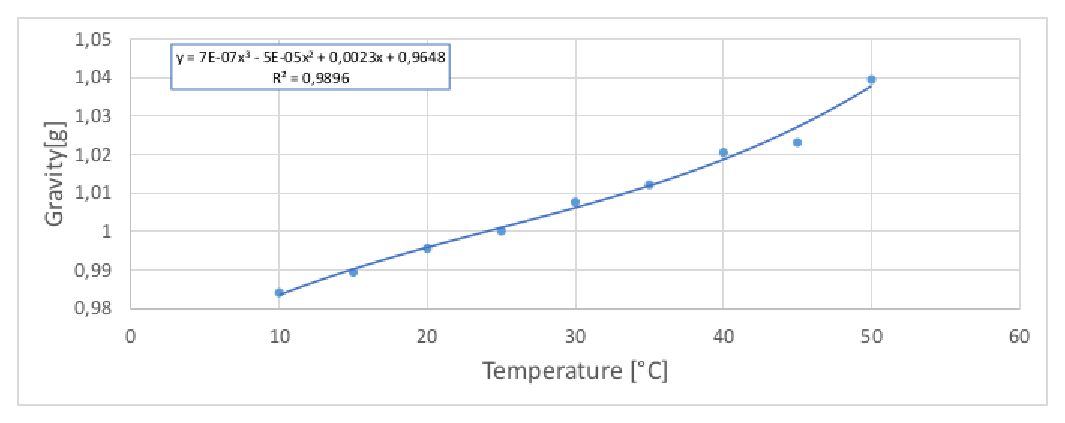
\includegraphics[width=0.45\textwidth]{Fig02.eps}
	\vspace{2.5cm}
	\caption{Gravity measurement in temperature range $10\degree C - 50\degree C$}
	\label{fig:imuTemp}
\end{figure}

Considering selected controllers, several hybrid data fusion approaches improving positioning accuracy can be found in literature. Authors have elaborated different approaches to fuse the sensors\' data which characterize various level of measurements reliability. First group of approaches can be classified as methods which use Kinect measurements as a reference system and partially relay on its measurements.\\
Bo et al. \cite{Bo2011} described the joint angle (angle between joint adjacent bones) estimation method exploiting 5 degrees of freedom (DOF) IMU and Kinect. The method initial stage interprets gyroscope and the accelerometer data separately and their fusion by the linear Kalman filter (KF) was subsequently performed. The same angle estimated with Kinect data was used to initially calibrate and then temporarily correct the bias of accelerometer estimation. There were no numerical results provided in the paper however presented charts suggest data fusion resulting considerable improvement.\\
A different approach was presented in a paper published by Destelle et al. \cite{Destelle2014}. Authors decided to use a set of 6DOF IMUs supported by magnetometer where each unit was sticked to one of the tracked limb bones. Basing on gathered measurements, orientation of each bone was estimated by Madgwick's algorithm \cite{Madgwick2010} and their superposition resulted in the full skeleton model. Kinect data was used twofold. The first stage was to get the initial, reference skeleton frame to ''label'' data, estimated from inertial units and improve the IMU calibration. That process resulted in hierarchical definition of bones orientations (''inertial skeleton''). The second stage of Kinect exploitation was to track position of central body point (torso joint) and then update the whole ''inertial skeleton'' relatively to this point displacement. Resulting, VICON referenced knee joints angle estimation error varied between $4\degree$ an $14\degree$. It depended on cross correlated joints, the measurements were referenced to, as there were no joints absolute angle estimation performed.\\
The newest method that could be qualified to this group is the one presented in 2015 by Tian et al. \cite{Tian2015}. Authors included in estimation process geometrical constraints of performed motion to eliminate estimations that are impossible to achieve in real life i.e. angle between forearm and arm cannot be greater than $180\degree$. Fusion algorithm used by authors based on Unscented Kalman Filter (UKF)\cite{Wan2000}. Presented results show that algorithm is able to work also while Kinect is outage, which was not obvious in previously described methods. To estimate method accuracy, authors compared elbow angle measurement. Authors published information that angle measurement estimated by their fusion method deviates from the expected value for less than 20 degree.\\
Another group of published methods based on the assumption that both measurement devices imperfections need to be corrected continuously by the signal fusion. In 2014 Feng and Murray-Smith \cite{Murray-Smith2014} proposed multi-rate Kalman filter based fusion method of joints positions, estimated by Kinect with linear acceleration and velocity of this joint. Presented results showed that this approach stabilizes measurements around real value much faster that single rate KF. This was visible especially when movemnt starts/stops (figure \ref{fig:feng-Stabilization}). The accuracy of presented method can be estimated around 1.5 -- 2cm (based on published diagrams). However presented results refer to very short time periods (up to 5s) so it is impossible to estimate how method works in a long time.\\

\begin{figure}[!htb]
	%\centering 
	%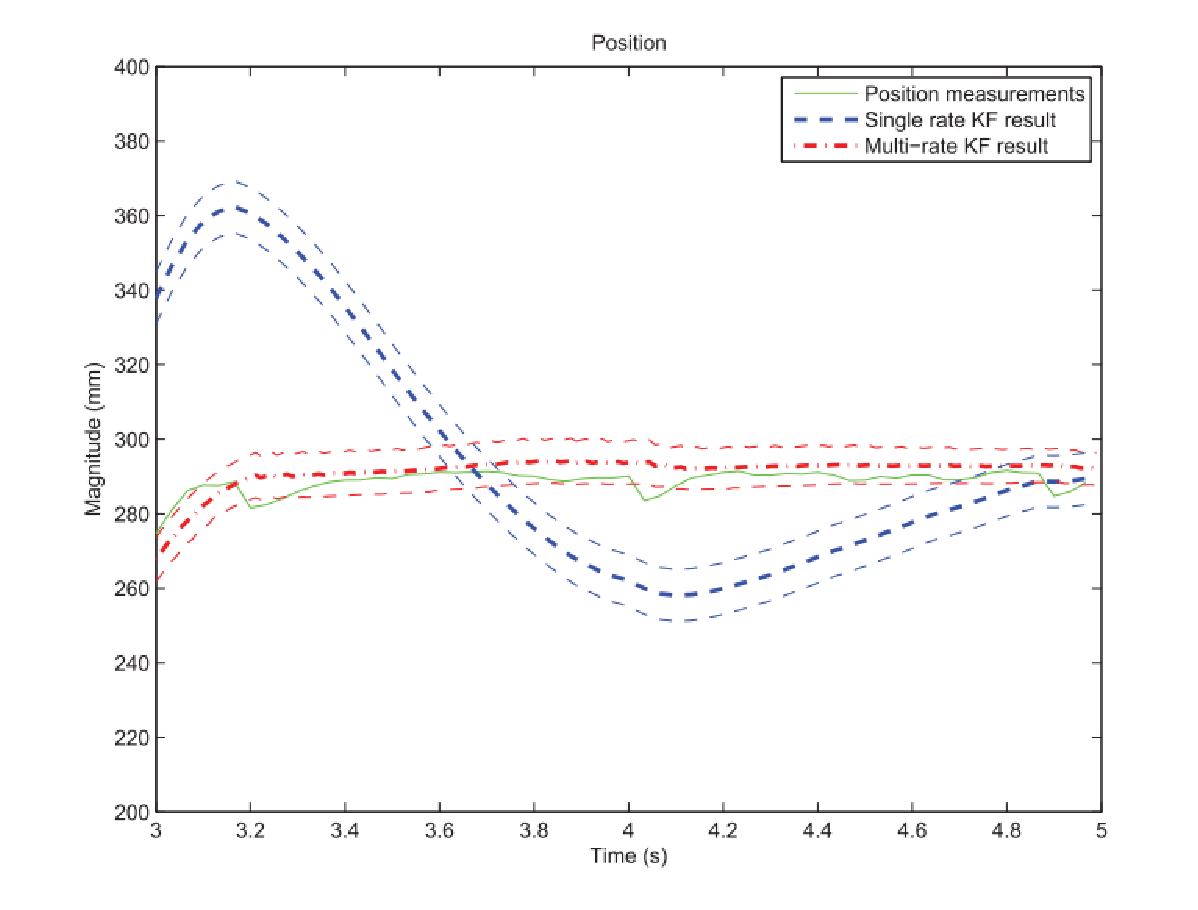
\includegraphics[width=0.45\textwidth]{Fig03.eps}
	\vspace{2.5cm}
	\caption{Joint position estimation with the multi-rate Kalman filter and the single rate Kalman filter\cite{Murray-Smith2014}. Red line - multi-rate Kalman filter, blue line - single-rate Kalman filter}
	\label{fig:feng-Stabilization}
\end{figure}

A different approach was presented in the paper of Kalkbrenner et al. \cite{Kalkbrenner2014}. Authors of this publication suggested Kalman based linear fusion of joints estimated positions retrieved from bones orientations superposed with skeleton model (bones length) and Kinect measurements. Absolute joints positions estimation results were around $\pm 2.5cm$ and seem to be the most accurate in long term experiments.\\
In the papers presented so far, motions described as test movements were performed in the ''Kinect friedly'' way. It means that all tracked joints were fully visible during all motion sequences and were done in the single axis that doesn\'t include any occlusions.\\
The approach presented in 2013 by Thomas Helten et al. \cite{Helten2013} is more advanced than methods presented so far and use pattern recognition to estimate current user's pose. In the previously analyzed articles, the IMU data was always fused with Kinect skeleton data and basing on that, multiple pose features were calculated. In the article, Kinect is used as a depth camera and data from the depth stream is fused with IMU measurements. The motion recording was performed with the use of six Xsens MTx 9 DOF IMUs \cite{XSense2015} which is a full set of professional inertial motion tracking system. The proposed method is based on the idea of the visibility model that is built from poses estimated on inertial and Kinect measurements, and then matched with predefined poses stored in the database. However, such approach seems to be useless in scenarios where you need to estimate joints positions and other limb features as it focuses on general pose recognition.\\
Our method is the most similar to the Kalkbrenner approach, but our main contribution consists in improved, weighted sensor contextual influence which results in overall better absolute joints positions estimations. The method joints absolute positioning precision of about 2-2.5 cm was verified against the ground-truth VICON system.


\section{Method}
A method, proposed by authors, bases on the continuous linear fusion of skeleton bones orientations with respect to the current motion context. It takes into consideration controllers reliability and compensates evaluation imperfections. The proposed motion positioning method can be defined as a function $f$:

\begin{equation}
	\label{eq:generalForm}
	f(A,G,T,P_0^K,P_1^K,Q^K,\Delta t) => [p_x^F,p_y^F,p_z^F]_t
\end{equation}
where:
\begin{itemize}
	\item $A$ -- accelerometer measurement
	\item $G$ -- gyroscope measurement
	\item $T$ -- temperature measurement
	\item $P_0^K,P_1^K$ -- start and end bone joints positions measured by Kinect i.e. elbow and wrist
	\item $Q^K$ -- bone orientation estimated by Kinect
	\item $t$ -- current time frame
	\item $\Delta t$ -- elapsed time between previous and current frame
\end{itemize}

Orientations are contextually presented in two forms: quaternions and Euler angles, and they are transformed between these forms with respect to North and South Pole singularities. In the method authors exploited limbs joints positions ($P^K=[p_x^K,p_y^K,p_z^K]$) and bones orientations ($Q^K=[q_w^K,q_x^K,q_y^K,q_z^K]$) supplied by the Kinect device as well as accelerometer ($A=[a_x,a_y,a_z]$), gyroscope ($G=[g_x,g_y,g_z]$) and temperature ($T$) measurements from each IMU. Kinect joints positions and IMU based marker locations on tracked limbs are presented in figure \ref{fig:skeleton}. \\
In the proposed method, data gathered from measurement devices, are denoised in the first step and then used to calculate bones orientations. Then, orientations calculated from IMU devices and measured by Kinect are fused together and at the last step, bones length model is added to estimate absolute joints positioins. General overview of orientation-based fusion process is presented on figure \ref{fig:orientationBasedMethod}.
 
\begin{figure}[!htb]
	%\centering 
	%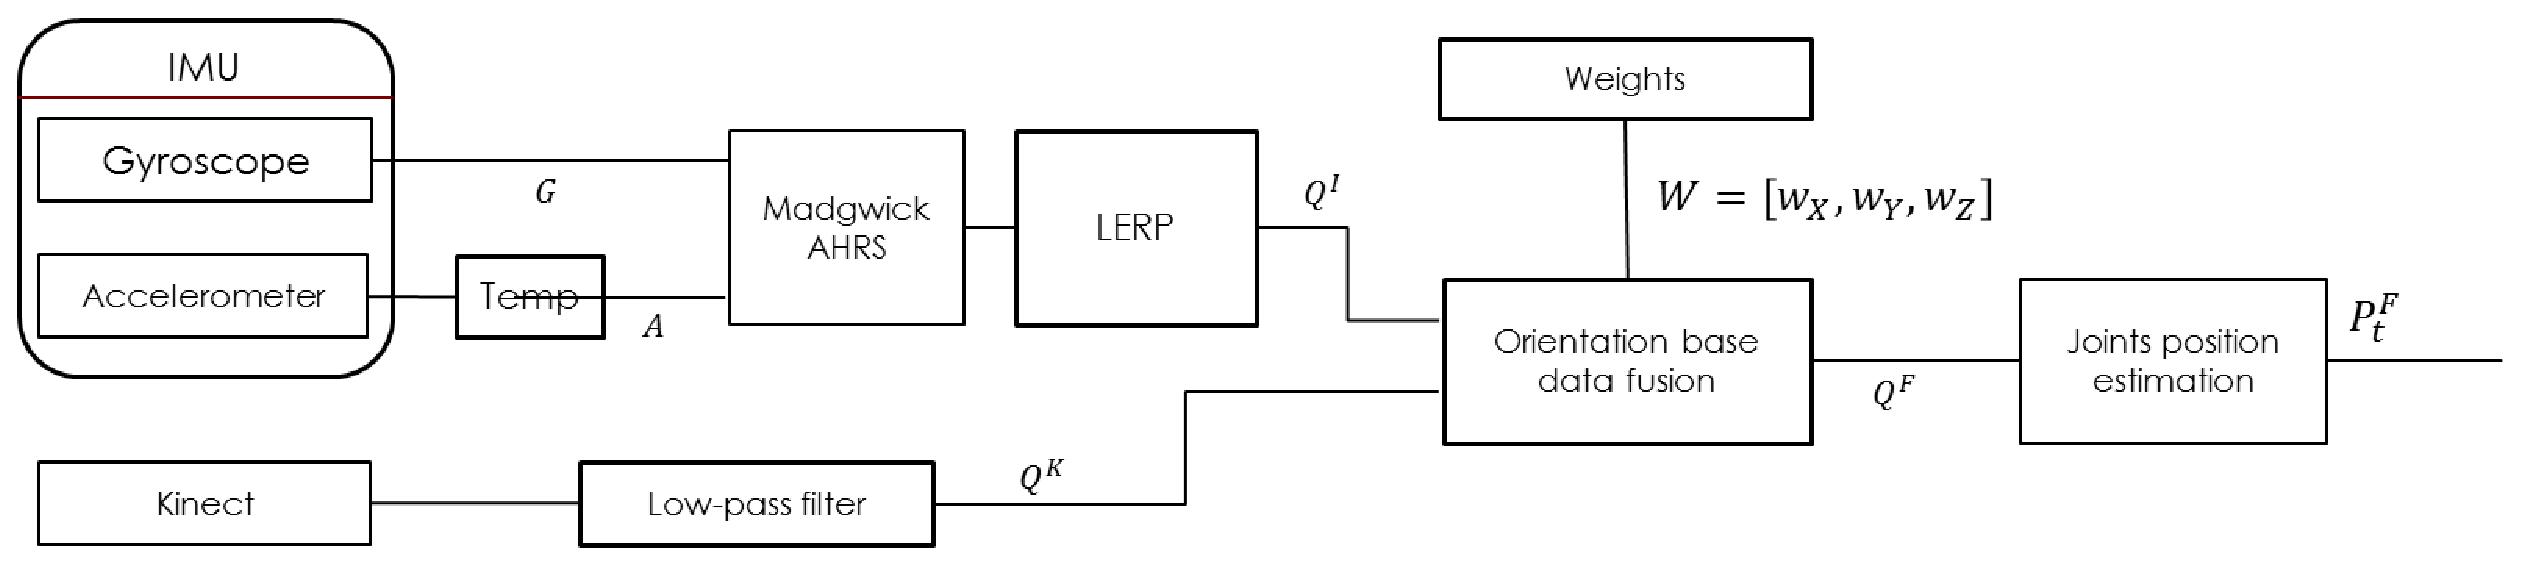
\includegraphics[width=0.9\textwidth]{Fig04.eps}
	\vspace{2.5cm}
	\caption{Orientation based fusion method}
	\label{fig:orientationBasedMethod}
\end{figure}

Data processing is performed in two parallel threads. The first one performs computations on the IMU data to estimate limbs orientations (quaternion) and the second retrieves Kinect skeleton bones orientations (quaternion). Their consequent, contextually weighted and time correlated, superposition results in fused bones quaternions values which, assuming skeleton model, can be transformed into estimated joints absolute positions.\\
At the beginning of the first thread, the IMU accelerometer bias was corrected with the equation \ref{eq:temperatureCompensation}, due to the device operating temperature destructive measurements influence.

\begin{equation}
	\label{eq:temperatureCompensation}
	A' = \frac{A}{1+\beta(T - T_0)}
\end{equation}
where:
\begin{itemize}
	\item $A'$ -- corrected accelerometer measurement
	\item $A$ -- accelerometer measurement
	\item $T$ -- temperature measurement
	\item $T_0$ -- device reference operating temperature. For used device $T_0 = 25\degree C$
	\item $\beta$ -- correction factor. For used device $\beta = 0.0011$
\end{itemize}

The value of $\beta$ correction factor was the result of exploited IMU gravity regression analysis as a function of the device operating temperature (figure \ref{fig:imuTemp}).
Next, the corrected accelerometer data and gyroscope measurements were used to calculate quaternion of adjacent bone orientation with Madgwick's filter \cite{Madgwick2010}. The estimated orientation was then extrapolated to eliminate the observed delay. The linear extrapolation algorithm was used in this step (equation \ref{eq:slerp}).
\begin{equation}
	\label{eq:slerp}
	[\Phi,\Theta,\Psi]' = [\Phi,\Theta,\Psi]_{t} + \gamma([\Phi,\Theta,\Psi]_{t} - [\Phi,\Theta,\Psi]_{t-1})
\end{equation}
where:
\begin{itemize}
	\item $[\Phi,\Theta,\Psi]'$ -- corrected orientation in the form of Euler angles
	\item $[\Phi,\Theta,\Psi]$ -- orientation in the form of Euler angles
	\item $\gamma$ -- extrapolation factor. For used device $\gamma = 0.5$
\end{itemize}

In the second thread, Kinect data needed to be denoised without the significant delay in measurements. It was done by first-order exponential low-pass filter defined by equation \ref{eq:lpf}. Both joint positions and orientations have been filtered in this step.
\begin{equation}
	\label{eq:lpf}
	y_t = \alpha x_t + (1-\alpha)y_{t-1}
\end{equation}
where:
\begin{itemize}
	\item $y$ -- filtered data
	\item $x$ -- noised data
	\item $\alpha$ -- filtration factor. $\alpha = 0.065$
\end{itemize}

The $\alpha$ factor value has been estimated as a result of the analysis of the average Kinect positioning error during hand motion sequence (presented in figure \ref{fig:lowPass}).

\begin{figure}[!htb]
	%\centering 
	%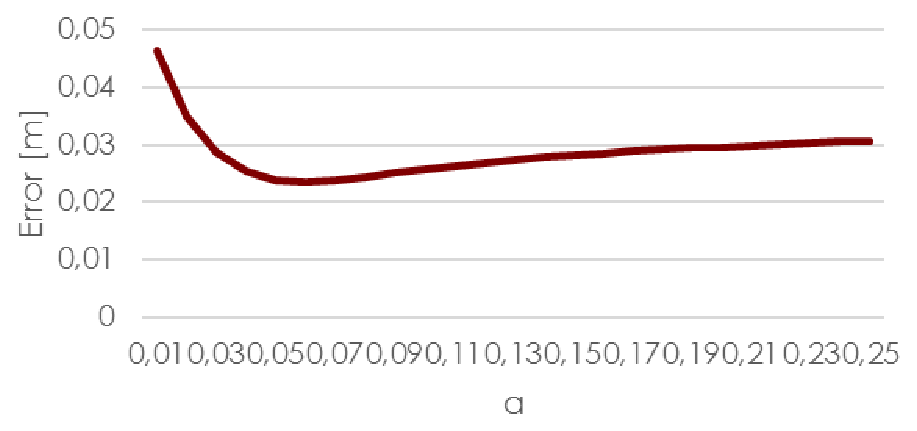
\includegraphics[width=0.45\textwidth]{Fig05.eps}
	\vspace{2.5cm}
	\caption{Kinect measurement accuracy to low-pass filter factor $\alpha$}
	\label{fig:lowPass}
\end{figure}

Both devices work in different coordination spaces (figure \ref{fig:coordinationSpaces}) and they need to be transformed into the common space before their data can be fused. As the majority of data is gathered from Kinect, its coordination space has been chosen as the main one. That minimizes additional computations that need to be done.

\begin{figure}[!htb]
	\centering 
	\begin{minipage}[b]{0.45\linewidth}
		\centering 
		
		%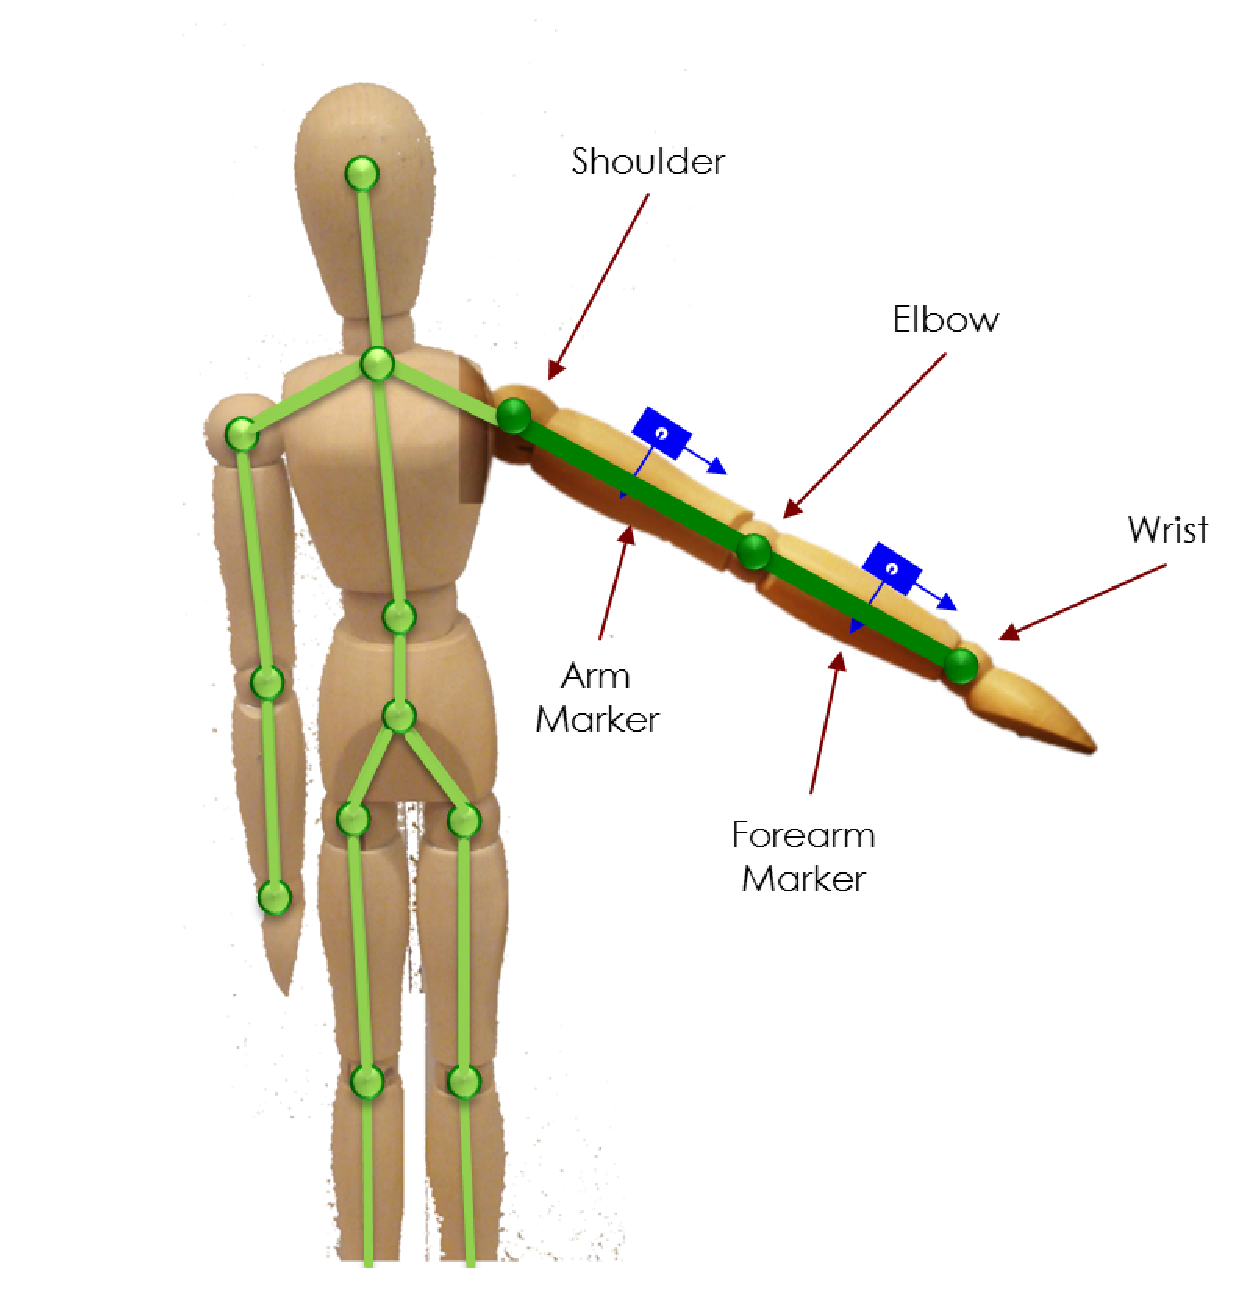
\includegraphics[width=\textwidth]{Fig06.eps}
		\vspace{2.5cm}
		\caption{Kinect skeleton joints positions and IMU location}
		\label{fig:skeleton}
	\end{minipage}
	\begin{minipage}[b]{0.45\linewidth}
		\centering 
		\subfigure[Kinect]
		{
			%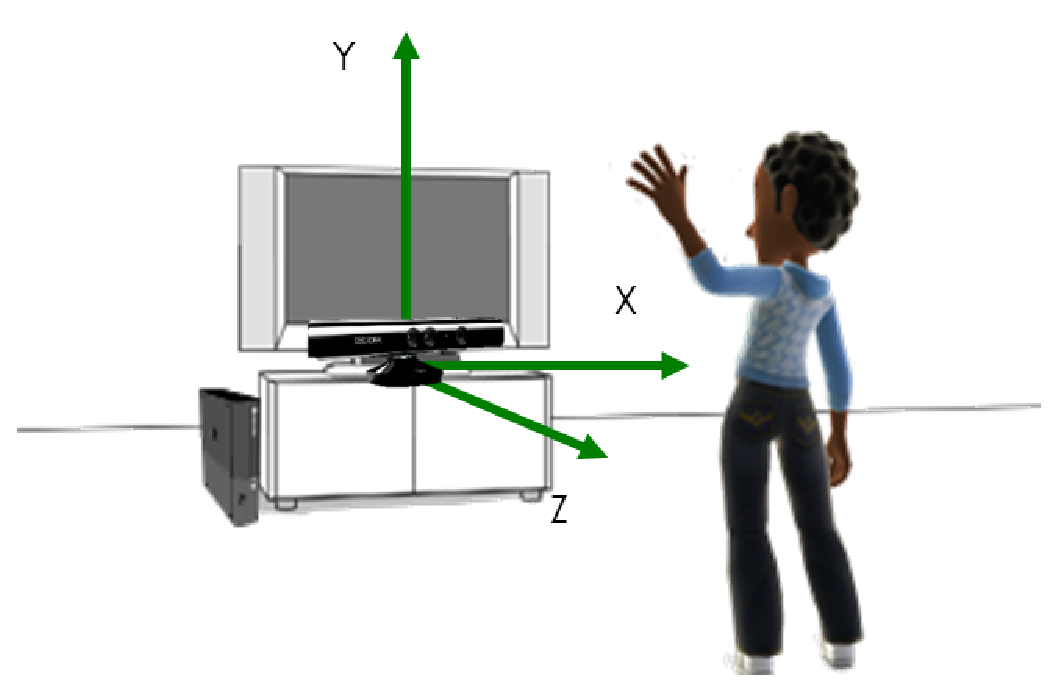
\includegraphics[width=40mm]{Fig07.eps}
			\vspace{2.5cm}
			\label{fig:kinectCoordinationSpace}
		}
		\subfigure[IMU]
		{
			%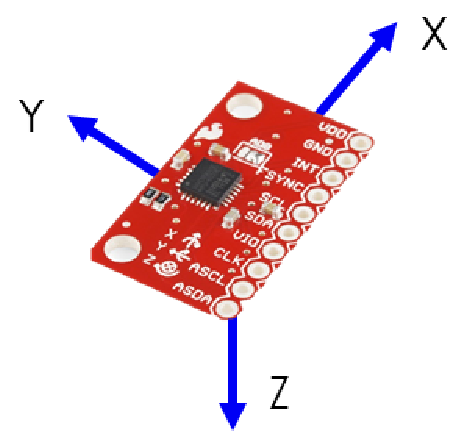
\includegraphics[width=25mm]{Fig08.eps}
			\vspace{2.5cm}
			\label{fig:imuCoordinationSpace}
		}
		\caption{Devices coordination spaces}
		\label{fig:coordinationSpaces}
	\end{minipage}
\end{figure}

In the next step, the controllers' quaternions fusion was performed. It started with the judgment of Kinect measurements reliability. The user orientation to the camera and joints positions measurement noise level were taken into consideration. The noise level is measured by the high-pass filter in the form of equation \ref{eq:hpf}. Sample results for keeping hands without motion and when Kinect lost tracking is presented on figure \ref{fig:hpfResults}.

\begin{equation}
	\label{eq:hpf}
	n_t = \delta n_{t-1} + \delta(P_t - P_{t-1}) 
\end{equation}\cite{HPFWiki}
where:
\begin{itemize}
	\item $n$ -- noise level
	\item $P$ -- joint position
	\item $\delta$ -- filtration factor. $\delta = 0.01$
\end{itemize}

\begin{figure}[!htb]
	\centering 
	\subfigure[Not occluded joint]
	{
		%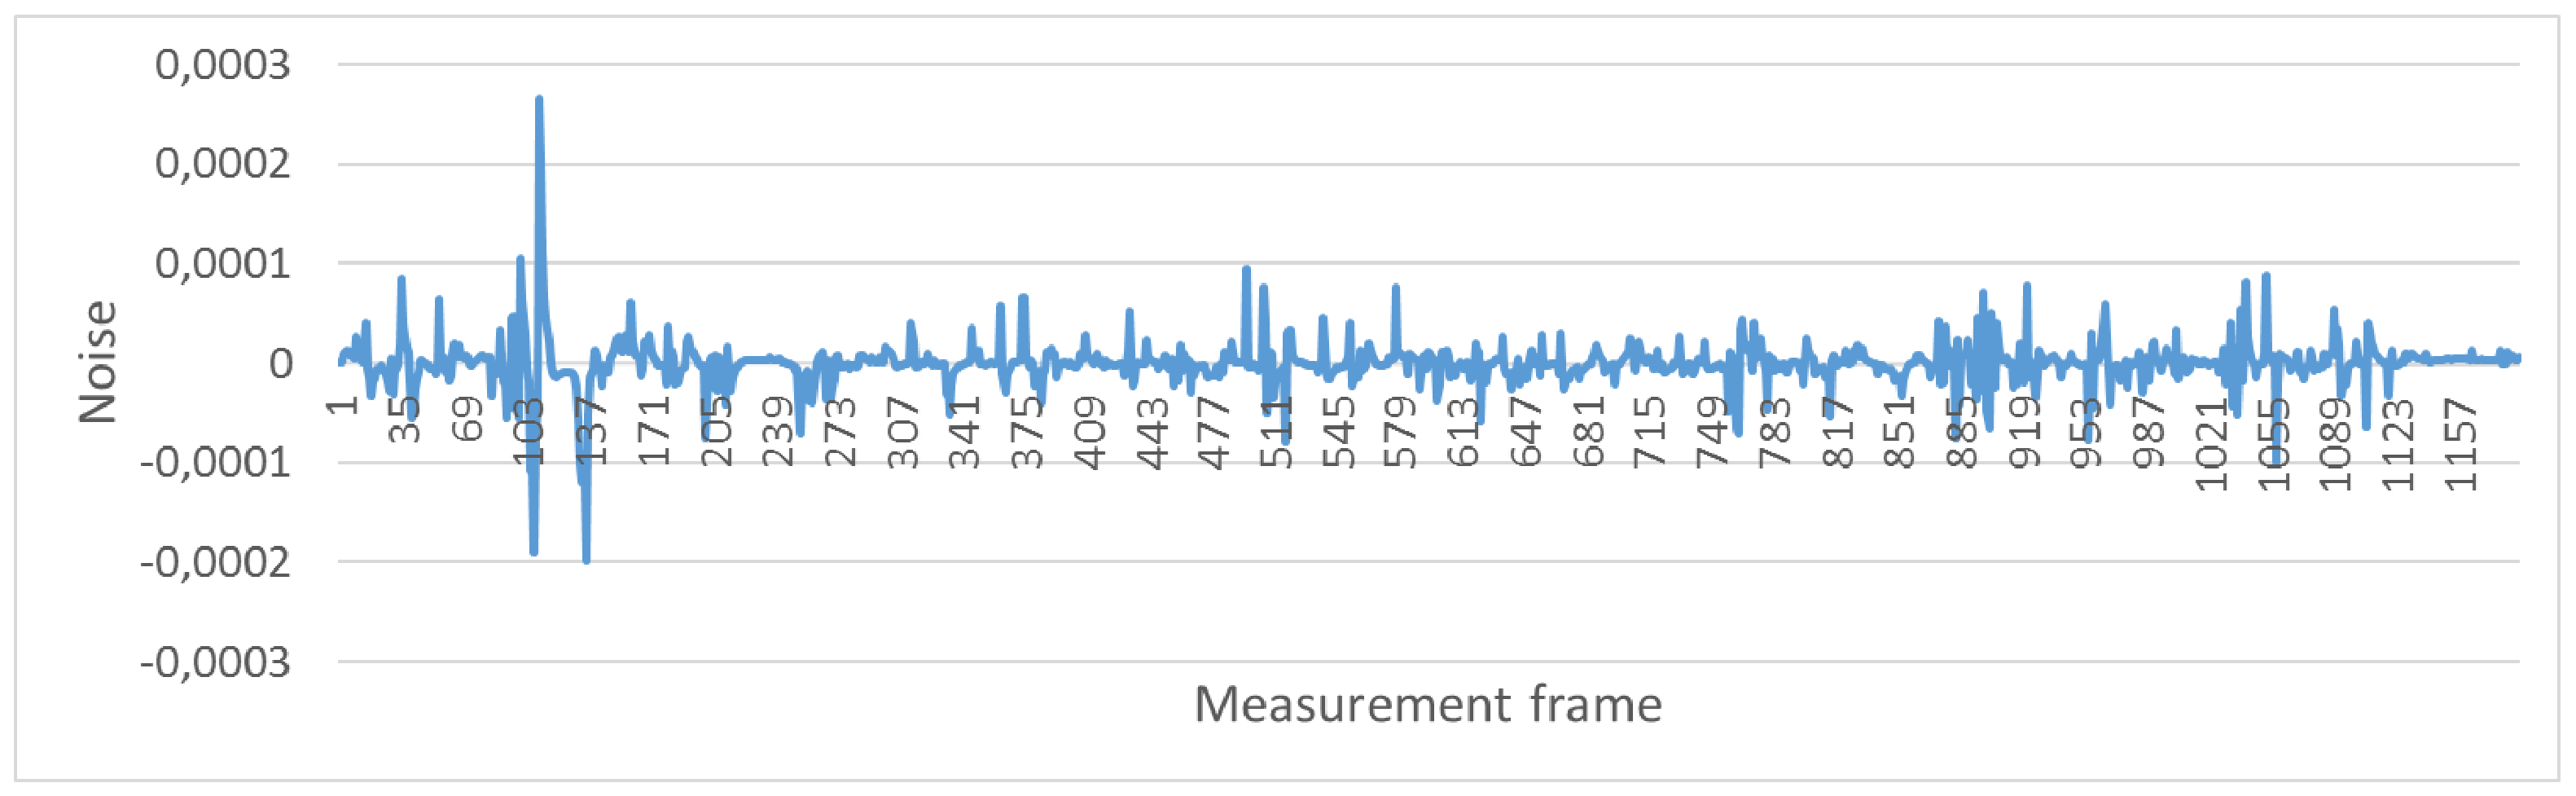
\includegraphics[width=0.45\textwidth]{Fig09.eps}
		\vspace{2.5cm}
		\label{fig:hpfNotOccluded}
	}
	\subfigure[Occluded joint]
	{
		%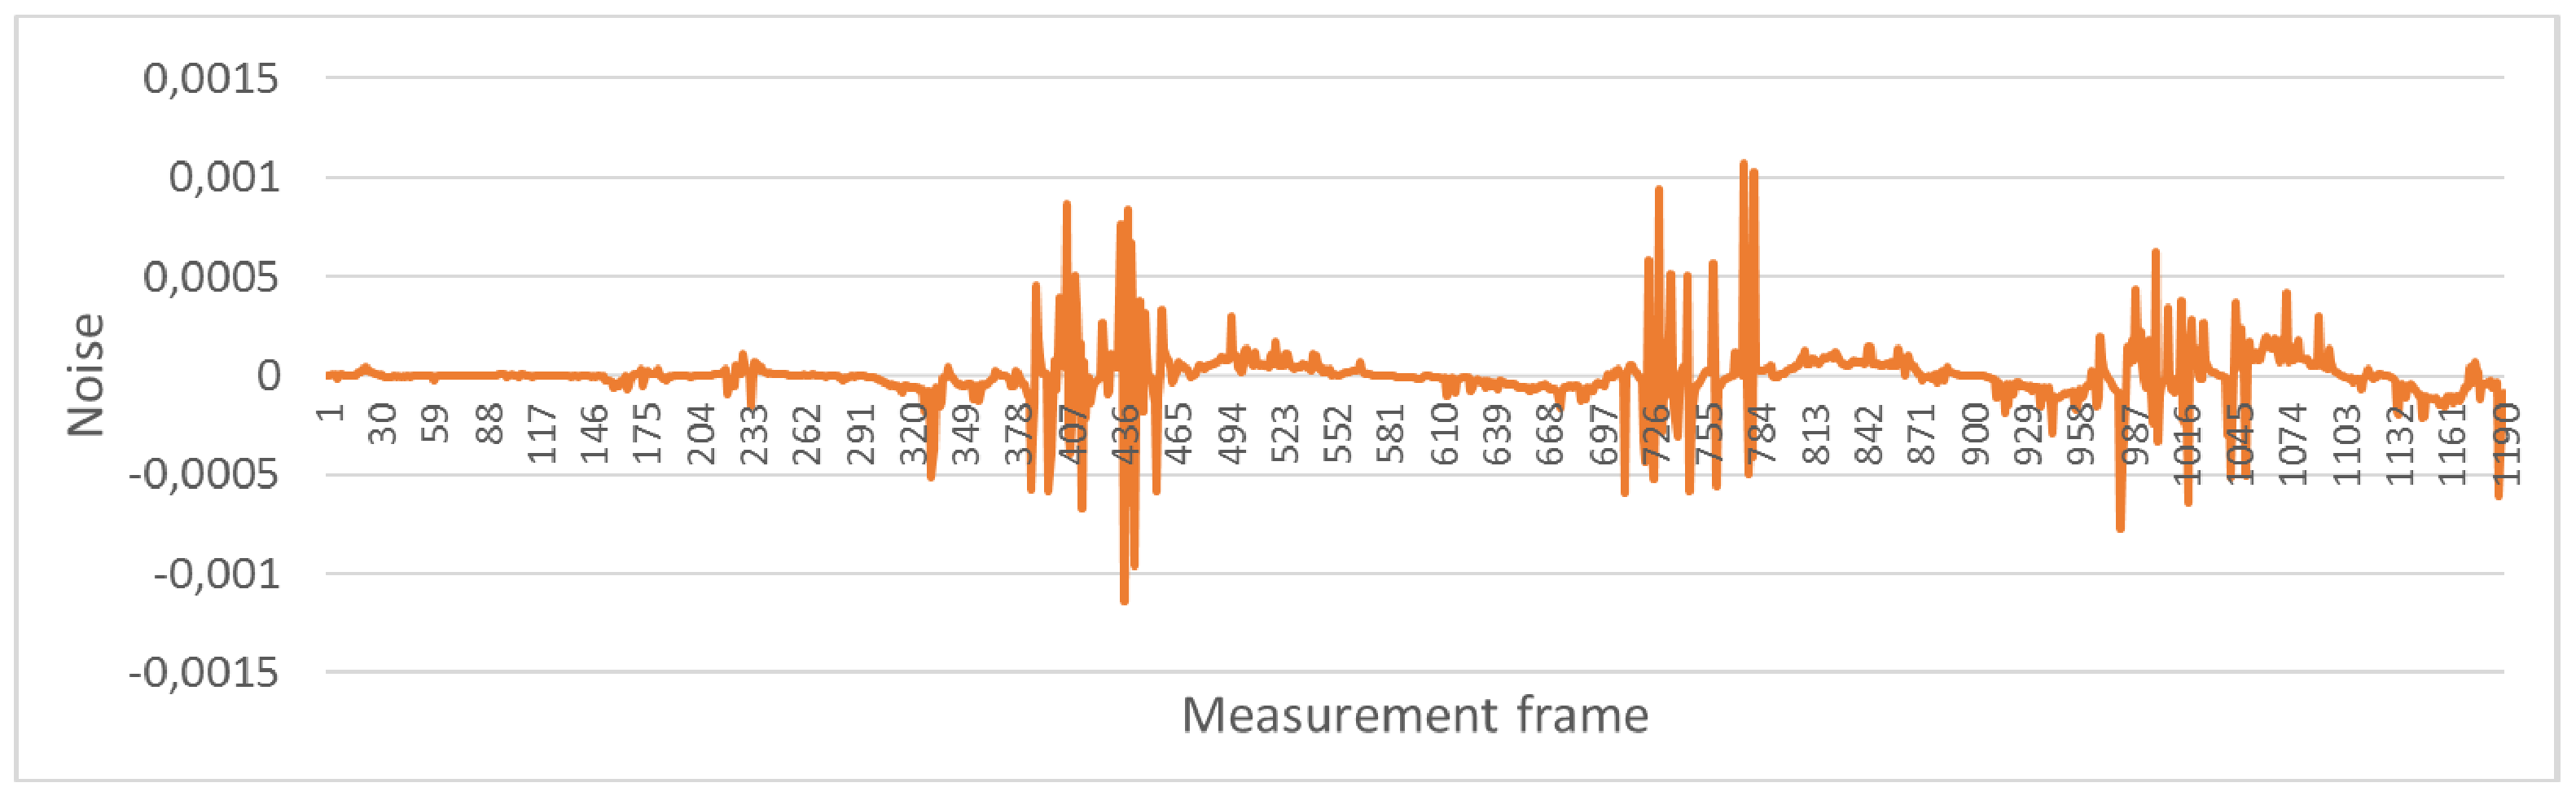
\includegraphics[width=0.45\textwidth]{Fig10.eps}
		\vspace{2.5cm}
		\label{fig:hpfOccluded}
	}
	\caption{High-pass filter (eq. \ref{eq:hpf}) results for joint position while joint is not occluded in any time (\ref{fig:hpfNotOccluded}) and partially occluded (\ref{fig:hpfOccluded})}
	\label{fig:hpfResults}
\end{figure}

If the user is rotated to Kinect camera more than $50\degree$ (the angle between line of user's shoulders and the camera surface) or the noise level is too high ($ |n| > 0.0004$ based on performed experiments) then Kinect measurements are classified as unreliable and are replaced with the difference between current and previous IMU--based orientation estimations. The orientations fusion is defined as the complementary process where rotations around each axis are joined with different weights. This approach was motivated by the fact that the controllers have different measurement abilities and accuracy in each axis.

If current Kinect's data is classified as reliable, the fusion is expressed by the following equation (eq. \ref{eq:reliableFusion}).

\begin{equation}
	\label{eq:reliableFusion}
	\begin{bmatrix}  \Phi^F \\  \Theta^F \\  \Psi^F \end{bmatrix}_t = 
	\begin{bmatrix}  w_x&0&0 \\  0&w_y&0 \\  0&0&w_z \end{bmatrix}
	\begin{bmatrix}  \Phi^I \\  \Theta^I \\  \Psi^I \end{bmatrix}_t + 
	\begin{bmatrix}  1-w_x&0&0 \\  0&1-w_y&0 \\  0&0&1-w_z \end{bmatrix}
	\begin{bmatrix}  \Phi^K \\  \Theta^K \\  \Psi^K \end{bmatrix}_t
\end{equation}
where:
\begin{itemize}
	\item $ \begin{bmatrix}  \Phi \\  \Theta \\  \Psi \end{bmatrix}_t$ -- Euler form-based orientation: \textbf{F} - fused, \textbf{I} - IMU, \textbf{K} - Kinect
	\item $w_x,w_y,w_z$ -- weights defined fusion factor of each axis rotation. Defines as $[0.98, 0.05, 0.65]$ respectively.
\end{itemize}

Weights used in equation \ref{eq:reliableFusion} describe the level of importance of IMU measurements and need to be $ < 1$. The higher value used, the more important measurement was. As Kinect is not able to measure rotation along 'x' axis (Roll), weight close to 1 has been used. In case of usage inertial sensors without magnetic sensor support, rotation around gravity vector ('y' axis -- Yaw) contains uncompensated time related drift so in this case IMU measurement was discriminated. Third axis rotation was measured by both devices, however IMU had slightly better accuracy than Kinect which was reflected in weight $ > 0.5$.

As both devices, Kinect and IMU, work with different sampling frequency, decimation technique has been used to pick the measurements from the closest time frames.

In case of Kinect data unreliability, the fusion was made between previously fused value and the IMU-based orientation update -- between the previous and the current measurements. The fusion formula is defined as follow (eq. \ref{eq:unreliableFusion}):
\begin{equation}
	\label{eq:unreliableFusion}
	\begin{bmatrix}  \Phi^F \\  \Theta^F \\  \Psi^F \end{bmatrix}_t = 
	\begin{bmatrix}  \Phi^F \\  \Theta^F \\  \Psi^F \end{bmatrix}_{t-1} + 
	\begin{bmatrix}  w_x&0&0 \\  0&w_y&0 \\  0&0&w_z \end{bmatrix}
	(\begin{bmatrix}  \Phi^I \\  \Theta^I \\  \Psi^I \end{bmatrix}_t -
	\begin{bmatrix}  \Phi^I \\  \Theta^I \\  \Psi^I \end{bmatrix}_{t-1})
\end{equation}
In this case $w_x$ value remains the same and it equals $0.98$ and $w_y$ and $w_z$ get low over the time according to the following function (eq. \ref{eq:weightCorrection}):
\begin{equation}
	\label{eq:weightCorrection}
	w = (1-\frac{\Delta t_n}{10}) * 0.65
\end{equation}
\begin{itemize}
	\item $w$ -- current weight value
	\item $\Delta t_n$ -- amount of time in seconds when Kinect stays unreliable.
\end{itemize}

When the controllers fused orientation was estimated it must be recalculated to the quaternion form. Then, basing on the known bone length, position of the desired joint might be calculated.

\section{Results}
In order to verify elaborated method (orientation-based joints position estimation) precision several experiments were performed. They were conducted with the VICON motion capture system as a source of a ground-truth reference data. Five users were monitored simultaneously with Kinect controller, two IMUs attached to hand arm and forearm bones (fig. \ref{fig:skeleton}) and passive marker-based VICON system. Markers were attached hand according to schema presented in figure \ref{fig:viconArm}.\\
\begin{figure}[H]
	%\centering
	%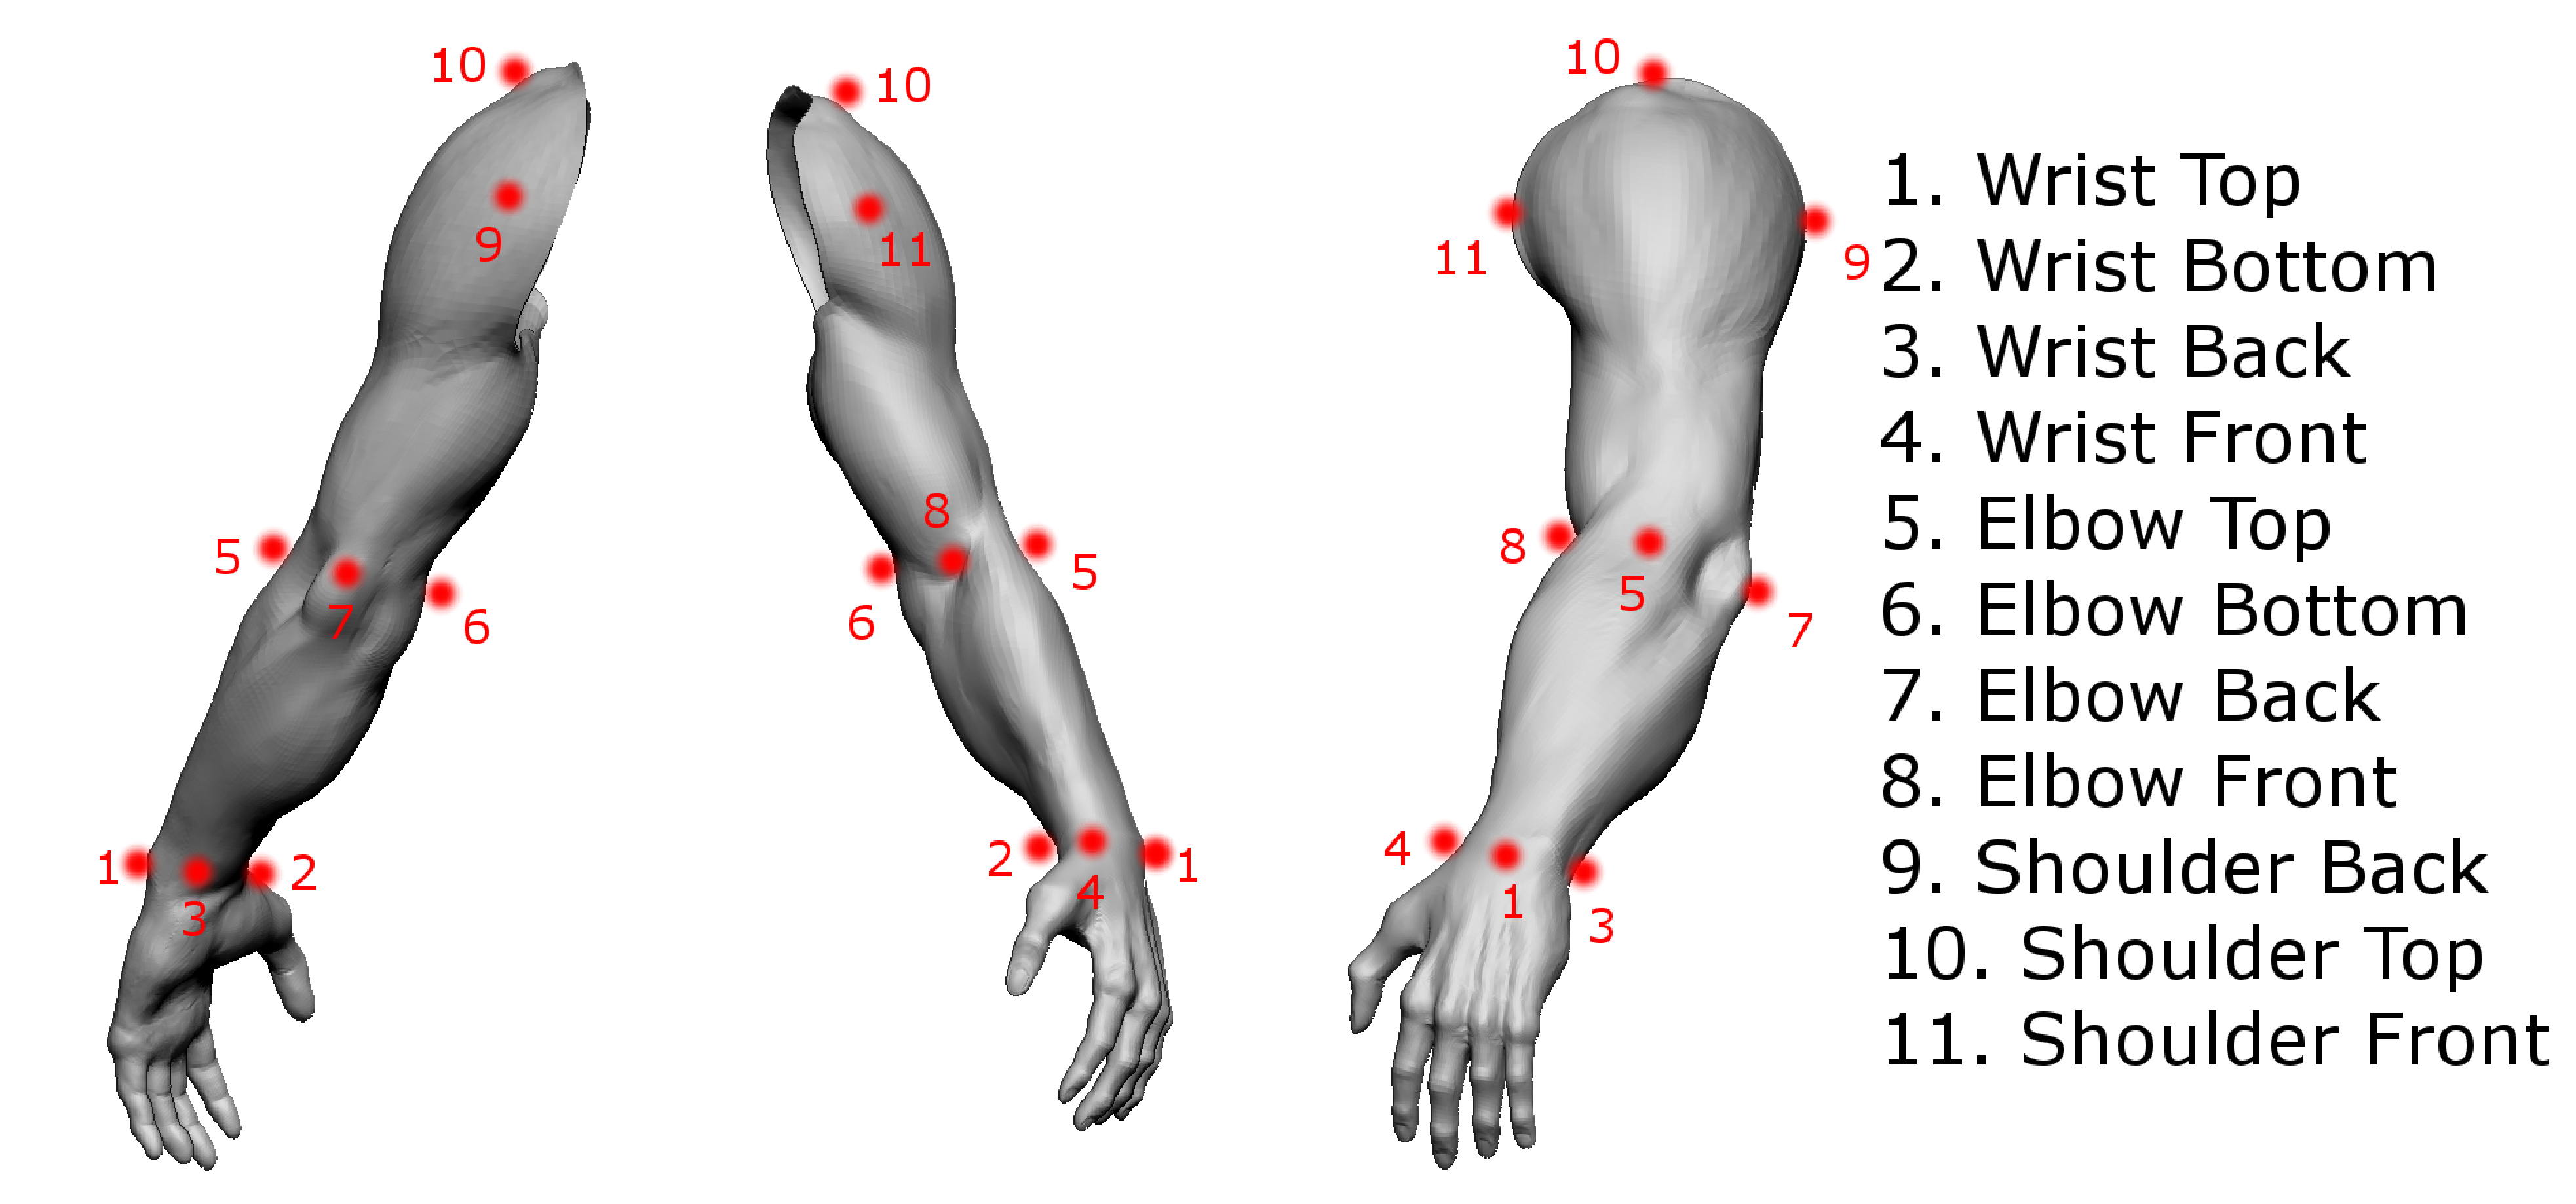
\includegraphics[width=0.6\textwidth]{Fig11.eps}
	\vspace{2.5cm}
	\caption[VICON arm marker schema]{Used VICON Arm marker model.\footnotemark}
	\label{fig:viconArm}
\end{figure}
The PC used to record Kinect and IMU data was a 2.5 GHz Intel Core i7-4710HQ CPU base computer with 8GB of RAM and SSD drive. The exploited Kinect device was a dedicated Xbox 360 console controller. The software was implemented on .Net Framework 4.5 with Kinect SDK v. 1.8. IMUs - these were MPU6050 devices set up with scale ranges: $\pm 4G$ for accelerometer and $\pm 500\degree /s$ for gyroscope. Inertial devices worked as a part of the self-made measurement device, built on the Arduino Due platform. The data transmission between IMUs and the PC was done through Bluetooth v. 2.0.\\
As a reference, measurements obtained from optical multicamera VICON motion capture has been used. Such systems are broadly used in the industry as well as to track the motion for i.e. biomechanical research \cite{ViconCaseStudeis}. According to data sheet published by the producer, declared precision of this system is down to $0.5mm$ of translatioin and $0.5\degree$ of rotation with refresh rate up to 250fps \cite{Vicon2016}. Such accuracy allows to use such measurements as ground-truth data. In performed experiments, VICON system worked with refresh rate 100 fps.\\
Performed experiments examined the right hand joints (elbow, wrist) positioning precision and the angle between the arm and the forearm estimation (the angle in the elbow joint) during 4 different movement sequences (fig. \ref{fig:poses}):
\begin{enumerate}
	\item Elbow flexion up to an angle of $90\degree$.
	\item Elbow flexion forward to an angle of $90\degree$.
	\item Straighten the hand in front of a body.
	\item Stand still for more than a minute.
\end{enumerate}

\begin{figure}[!htb]
	%\centering
	%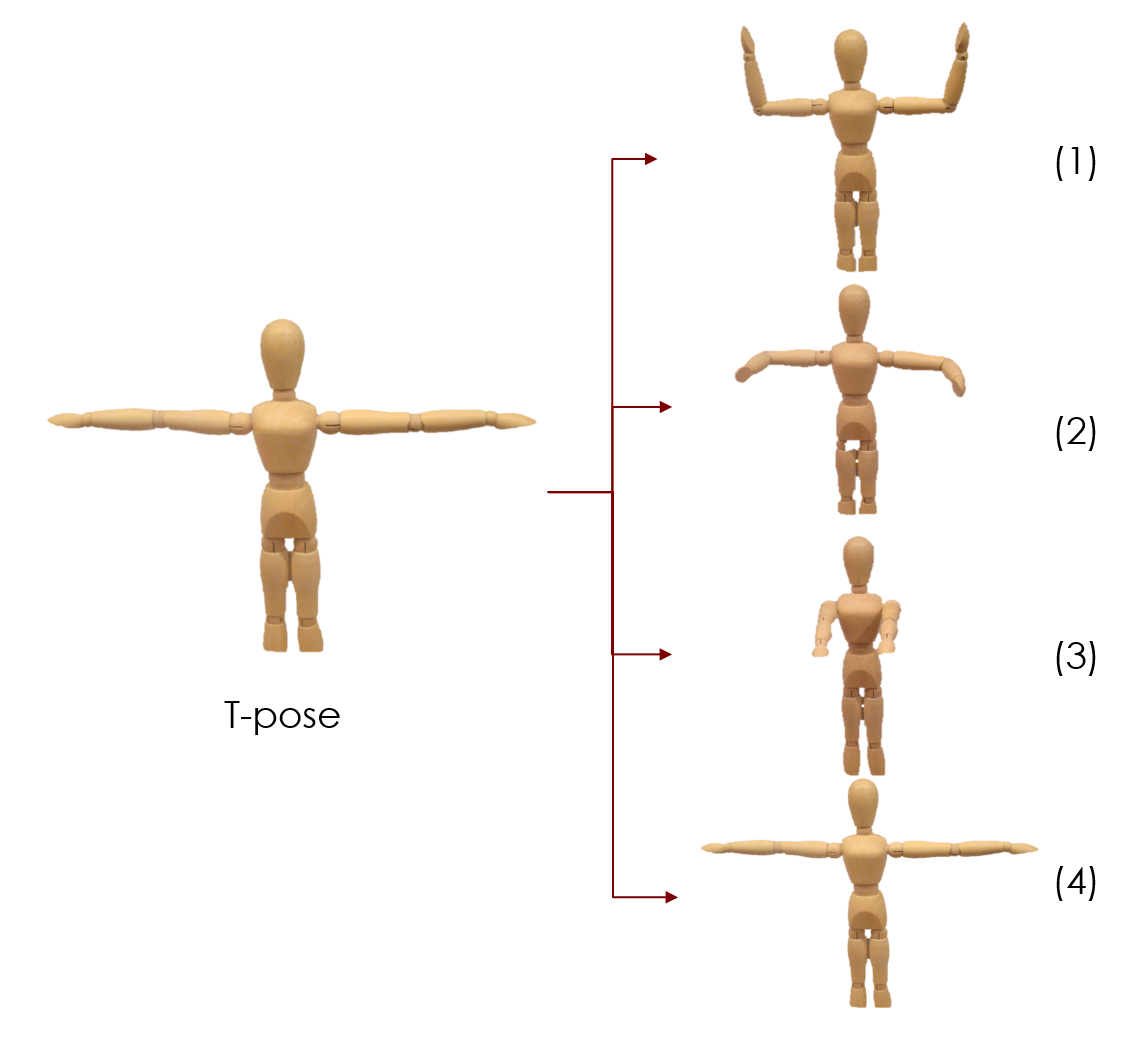
\includegraphics[width=0.35\textwidth]{Fig12.eps}
	\vspace{2.5cm}
	\caption{Movement sequences performed during tests.}
	\label{fig:poses}
\end{figure}

\footnotetext{Arm's render author: Pranay P. Pai. Source: \cite{Pranay2013}}

Selected gestures comprised motions that might be considered as challenging especially for Kinect. Each of movement sequences started from the initial T-pose and were performed multiple times and averaged. 
The proposed method was also compared with the Kalkbrener method precision, which was implemented according to the description included in the article \cite{Kalkbrenner2014}. 
The position estimation accuracy for elbow and wrist joints as well as the angle measurement accuracy has been presented in figures \ref{fig:positionElbow}, \ref{fig:positionWrist} and \ref{fig:angleError}. The grey color was used for Kalkbrener, position-based, method results and the orange for the author's, orientation-based, method achievements. Unfortunately, during performed tests, authors were not able to achieve the described accuracy for the Kalkbrner position-based method, however achieved results were close to the declared ones. Results presented on charts show the improvement in both: the position and the angle measurement accuracy. The average accuracy for the position estimation was $2.5 cm$ for the elbow and $2.9 cm$ for the wrist. The average angle measurement accuracy was $2.5\degree$. The same values for position-based fusion estimations were $2.8 cm, 3.6 cm$ and $5.9\degree$ respectively.

\begin{figure}[!htb]
	\centering
	\begin{minipage}[b]{0.49\linewidth}
		\centering   
		%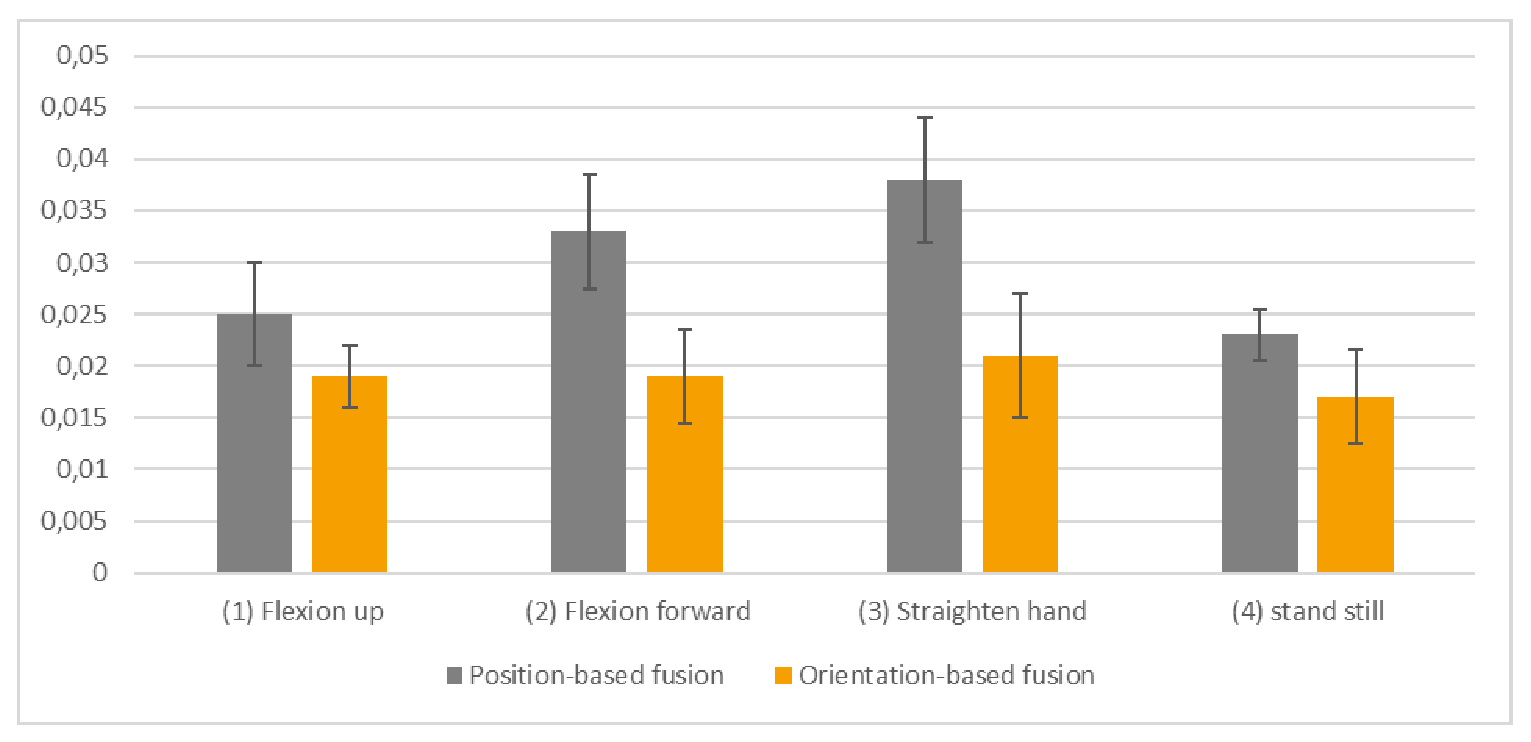
\includegraphics[width=\textwidth]{Fig13.eps}
		\vspace{2.5cm}
		\caption{Elbow positioning average accuracy}
		\label{fig:positionElbow}
	\end{minipage}
	\begin{minipage}[b]{0.49\linewidth}
		\centering 
		%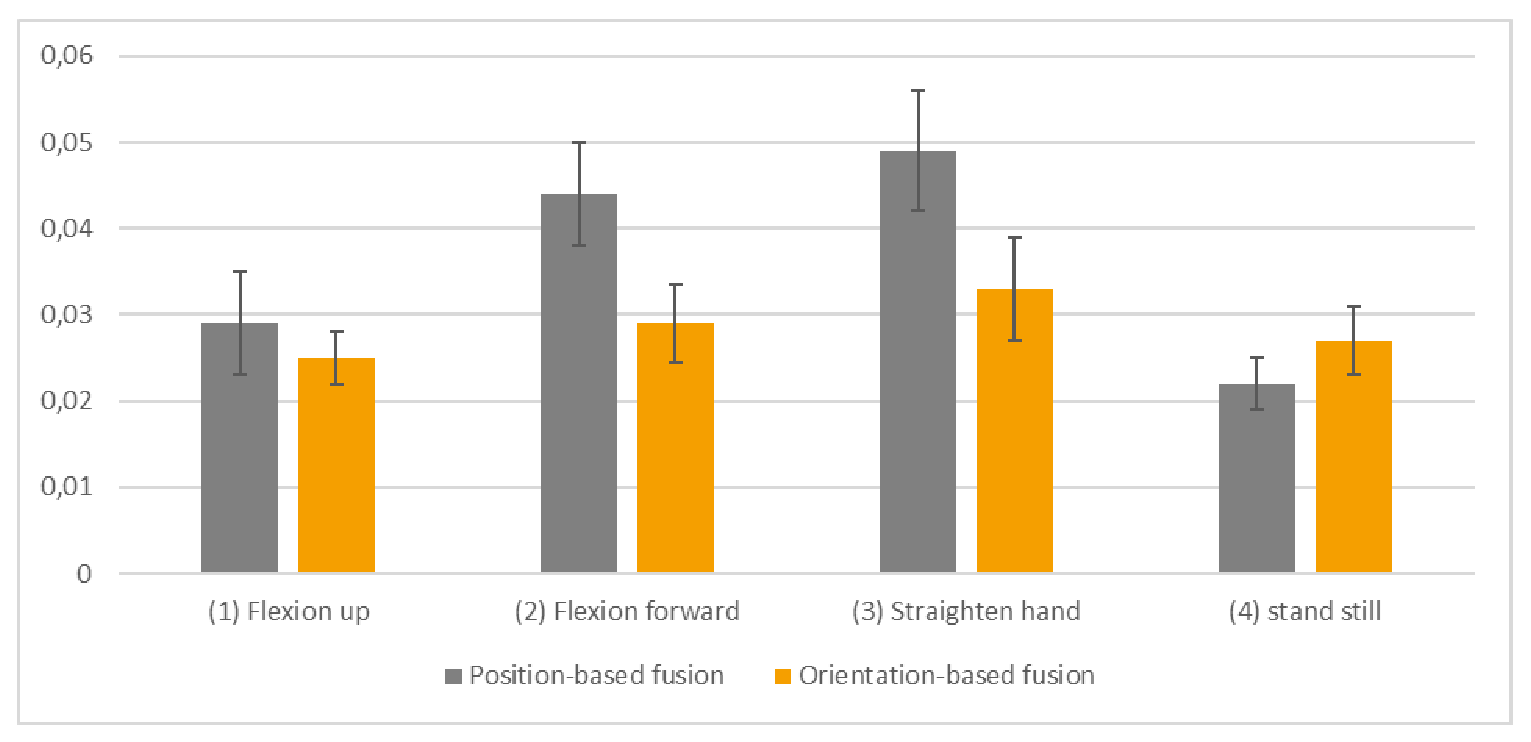
\includegraphics[width=\textwidth]{Fig14.eps}
		\vspace{2.5cm}
		\caption{Wrist positioning average accuracy}
		\label{fig:positionWrist}
	\end{minipage}
	
\end{figure}

\begin{figure}[!htb]
	%\centering 
	%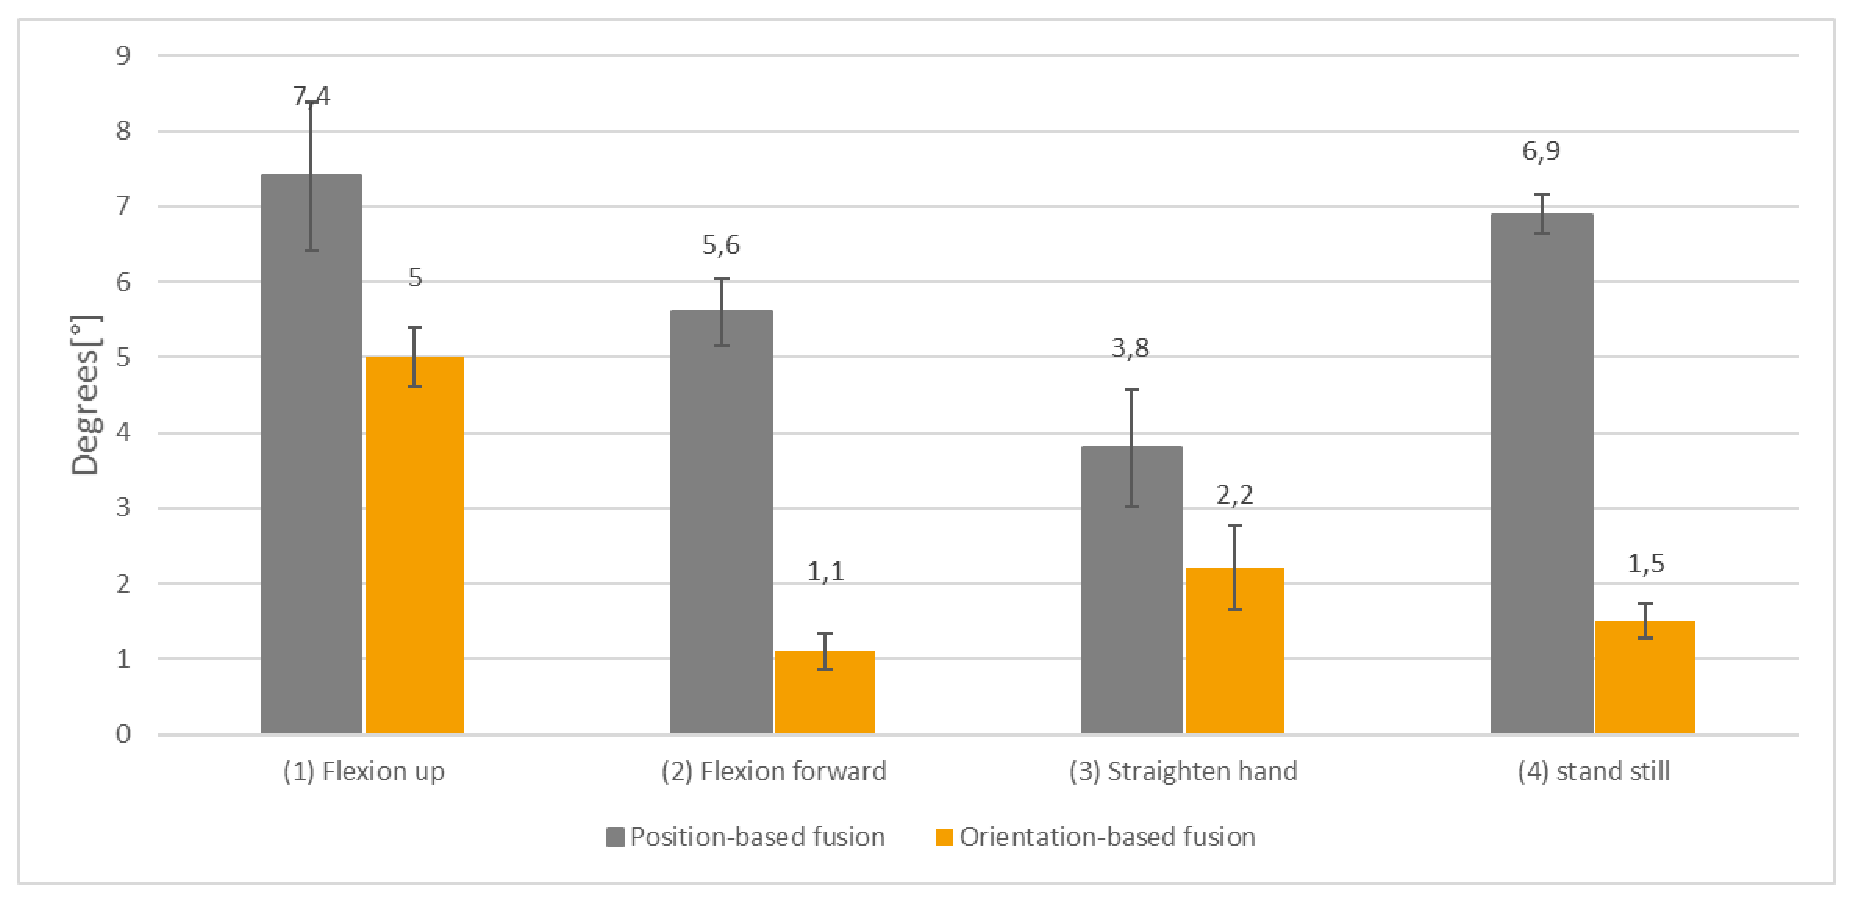
\includegraphics[width=0.45\textwidth]{Fig15.eps}
	\vspace{2.5cm}
	\caption{Elbow angle measurement average accuracy}
	\label{fig:angleError}
\end{figure}

\section{Conclusion}
The authors presented a new, orientation-based, method for skeleton joints positioning. It was tested on variety of right hand movements. Obtained results have prooved that the method managed to compensate imperfections of both measurement devices much better than previous approaches. Basing on the comparison of results gathered from the orientation-based fusion and the position-based fusion, the improvement of the estimation accuracy has been noticed and reached the rate of 15\% up to 25\% precision improvement. \\
Obtained results proof that the novel data fusion approach based on the bones orientation might be considered as an improved alternative to the well known, joint position-based methods.

\begin{thebibliography}{9}
	%6
	\bibitem {Kalkbrenner2014}
	Kalkbrenner, Christoph et al:
	Motion Capturing with Inertial Measurement Units and Kinect - Tracking of Limb Movement using Optical and Orientation Information.
	Proceedings of the International Conference on Biomedical Electronics and Devices (2014)
	%1
	\bibitem {Bo2011}
	Bo, Antonio Padilha Lanari et al:
	Joint angle estimation in rehabilitation with inertial sensors and its integration with Kinect.
	Proceedings of the Annual International Conference of the IEEE Engineering in Medicine and Biology Society, EMBS/2011 (2011)
	%2
	\bibitem {Destelle2014}
	Destelle, F. et al: 
	Low-cost accurate skeleton tracking based on fusion of kinect and wearable inertial sensors.(2014)
	%5
	\bibitem {Murray-Smith2014}
	Feng, Shimin and Murray-Smith, Roderick:
	Fusing Kinect Sensor and Inertial Sensors with Multi-rate Kalman Filter.
	IET Conf. Data Fusion Target Track. 2014 Algorithms Appl. (2014)
	%8
	\bibitem {Asteriadis2013}
	Asteriadis, Stylianos et al:
	Estimating human motion from multiple Kinect sensors
	Proc. 6th Int. Conf. Comput. Vis. / Comput. Graph. Collab. Tech. Appl. - MIRAGE '13 (2013)
	%9
	\bibitem {Khoshelham2012}
	Khoshelham, Kourosh and Elberink, Sander Oude:
	Accuracy and Resolution of Kinect Depth Data for Indoor Mapping Applications.
	Sensors (2012)
	%10
	\bibitem{Woodman2007}
	Woodman, Oliver J.:
	An introduction to inertial navigation
	University of Cambridge Technical Report, Vol. 696 (20070
	%11
	\bibitem{Nikolic2013}
	Renaut, Felix and Nikolic, Janosh:
	MEMS Inertial Sensors Technology (2013)
	%12
	\bibitem{Obdrzalek2012}
	Obdrz{\'{a}}lek, Step{\'{a}}n et al:
	Accuracy and robustness of Kinect pose estimation in the context of coaching of elderly population.
	Engineering in Medicine and Biology Society (EMBC), 2012 Annual International Conference of the IEEE (2012)
	%4
	\bibitem {Madgwick2010}
	Madgwick, S.O.H.:
	An efficient orientation filter for inertial and inertial/magnetic sensor arrays. (2010)
	%13
	\bibitem{Tian2015}
	Tian, Yushuang et al:
	Upper limb motion tracking with the integration of IMU and Kinect
	Neurocomputing (2015)
	%14
	\bibitem{Wan2000}
	Wan, E.A. and {Van Der Merwe}, R.:
	The unscented Kalman filter for nonlinear estimation
	Proc. IEEE 2000 Adapt. Syst. Signal Process. Commun. Control Symp. (Cat. No.00EX373 (2000)
	%7
	\bibitem {Helten2013}
	Helten, Thomas et al:
	Real-time body tracking with one depth camera and inertial sensors.
	Proc. IEEE Int. Conf. Comput. Vis. (2013)
	%17
	\bibitem{XSense2015}
	XSense:
	MTx--Products--Xsens 3D motion tracking.[Online]. 
	Available: https://www.xsens.com/products/mtx/. [Accessed: 10-Nov-2015].
	%20
	\bibitem{HPFWiki}
	Wikipedia contributors:
	High-pass filter --- Wikipedia, The Free Encyclopedia,
	https://en.wikipedia.org/wiki/High-pass\_filter\#Algorithmic\_implementation [Accessed: 01-Jan-2016]
	%19
	\bibitem{Pranay2013}
	Pranay P Pai: 
	Human Male Sculpt (Maya and Zbrush Pipeline) 
	Available: http://graphyx-medley.blogspot.com/2013/07/human-male-sculpt.html [Accessed: 01-Jan-2016]
	%
	\bibitem{ViconCaseStudies}
	Vicon:
	Case Studies | VICON
	Availabel: http://www.vicon.com/case-studies [Accessed: 12-Feb-2016]
	%
	\bibitem{Vicon2016}
	Vicon:
	Bonita Motion Capture Camera  | VICON
	Available: http://www.vicon.com/products/camera-systems/bonita [Accessed: 12-Feb-2016]
	
\end{thebibliography}

\end{document}
